\chapter{評価手法と結果}
\label{chap:evaluation}
\section{本提案の評価概要と予想}
\ref{subsection:要件1}で述べた通り、リンク障害による配送遅延の増加の発生後、
Contact Planの臨時更新を行うと、そのリンク情報がすべてのノードに伝搬し
再計算が行われる時間の間、一時的にContact Planの不整合が発生する。

\section{シミュレーション結果}
本章では、\ref{chap:implementation_and_experimentation}で
述べたシミュレーションにおける結果についてまとめる。
\ref{subsection:経路収束までの所要時間}では、
\ref{subsection:要件1}で述べた経路収束までの所要時間についての
シミュレーション結果について、\ref{subsection:経路収束後の到達遅延}では
\ref{subsection:要件2}で述べた経路収束後の配送遅延についての
シミュレーション結果について述べる。


\subsection{経路収束までの所要時間}
\label{subsection:経路収束までの所要時間}
\ref{subsection:要件1}で述べた通り、リンク障害による配送遅延の増加の発生後、
Contact Planの臨時更新を行うと、そのリンク情報がすべてのノードに伝搬し
再計算が行われる時間の間、一時的にContact Planの不整合が発生し、経路収束までの所要時間の
間は遅延が大きくなることが予想される。
\begin{figure}[tbh]
    \centering
    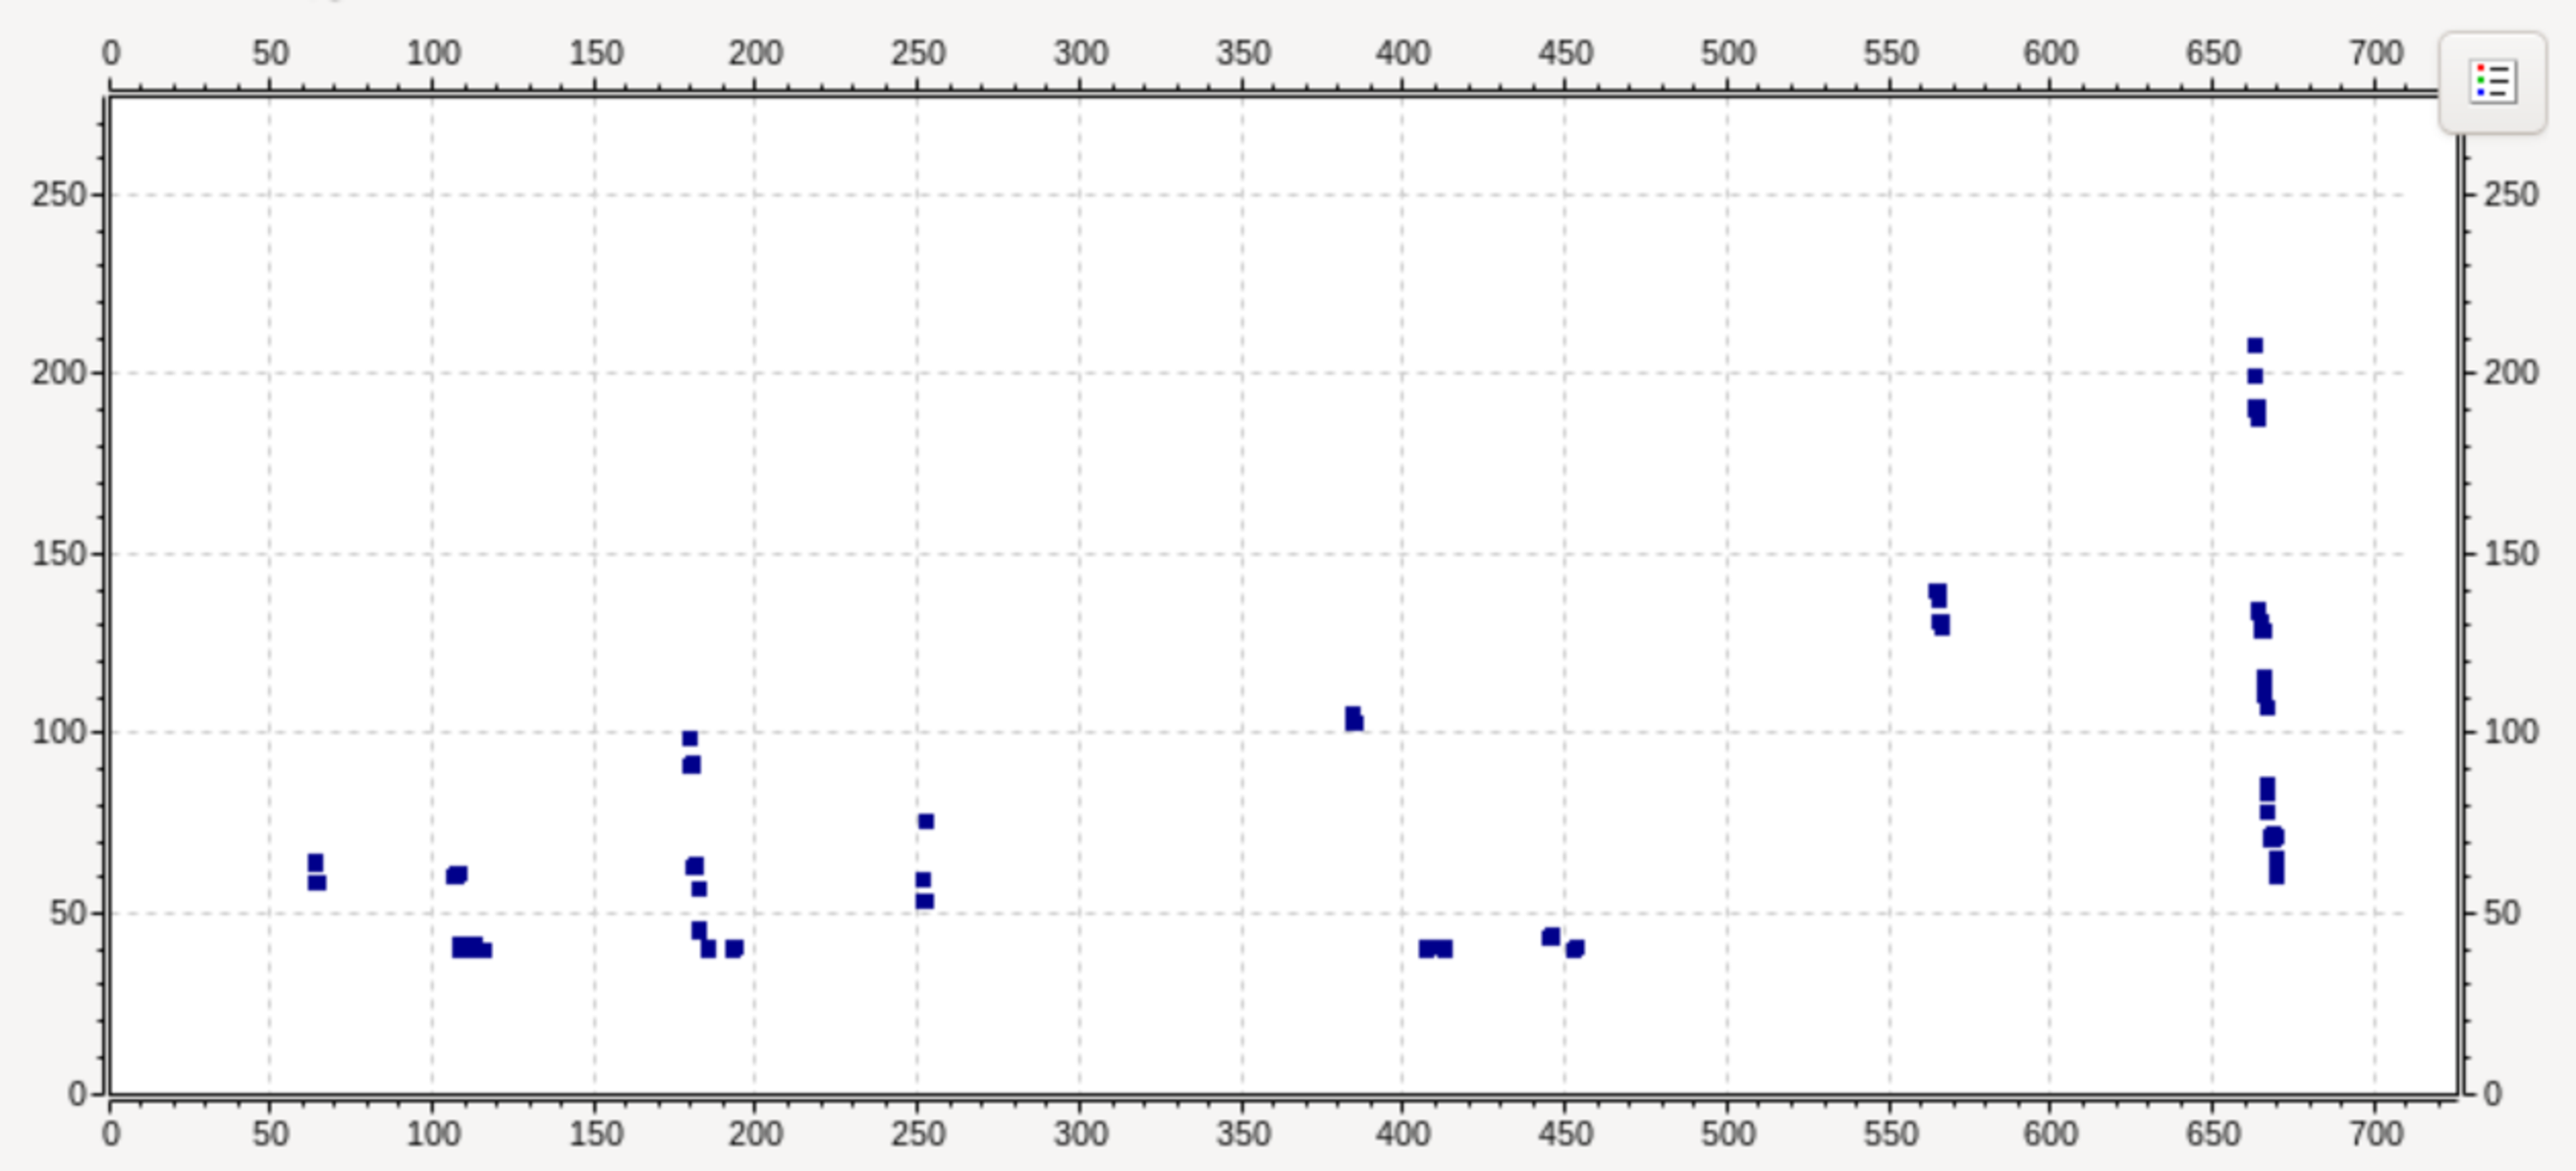
\includegraphics[width=0.7\textheight]{img/thesis_sample_delay_time.pdf}
    \caption{ノード6に向けたBundleの到達遅延の時間変化(地球・月間のシミュレーション)}
    \label{fig:delay_time_variation_earth_moon}
    \begin{minipage}{\textwidth}
        \raggedright
        \vspace{3mm}
        ノード6における、シミュレーション内での全到達Bundleの到達遅延の最大値・平均値・最小値。
        本シミュレーションにおいては、\ref{subsection:シミュレーションで用いるバンドルトラフィック}
        で述べたように、ノード6に対するBundleトラフィックのみを生成しているため、
        ノード6のみの到達遅延を示す。
    \end{minipage}
\end{figure}

\begin{figure}[tbh]
    \centering
    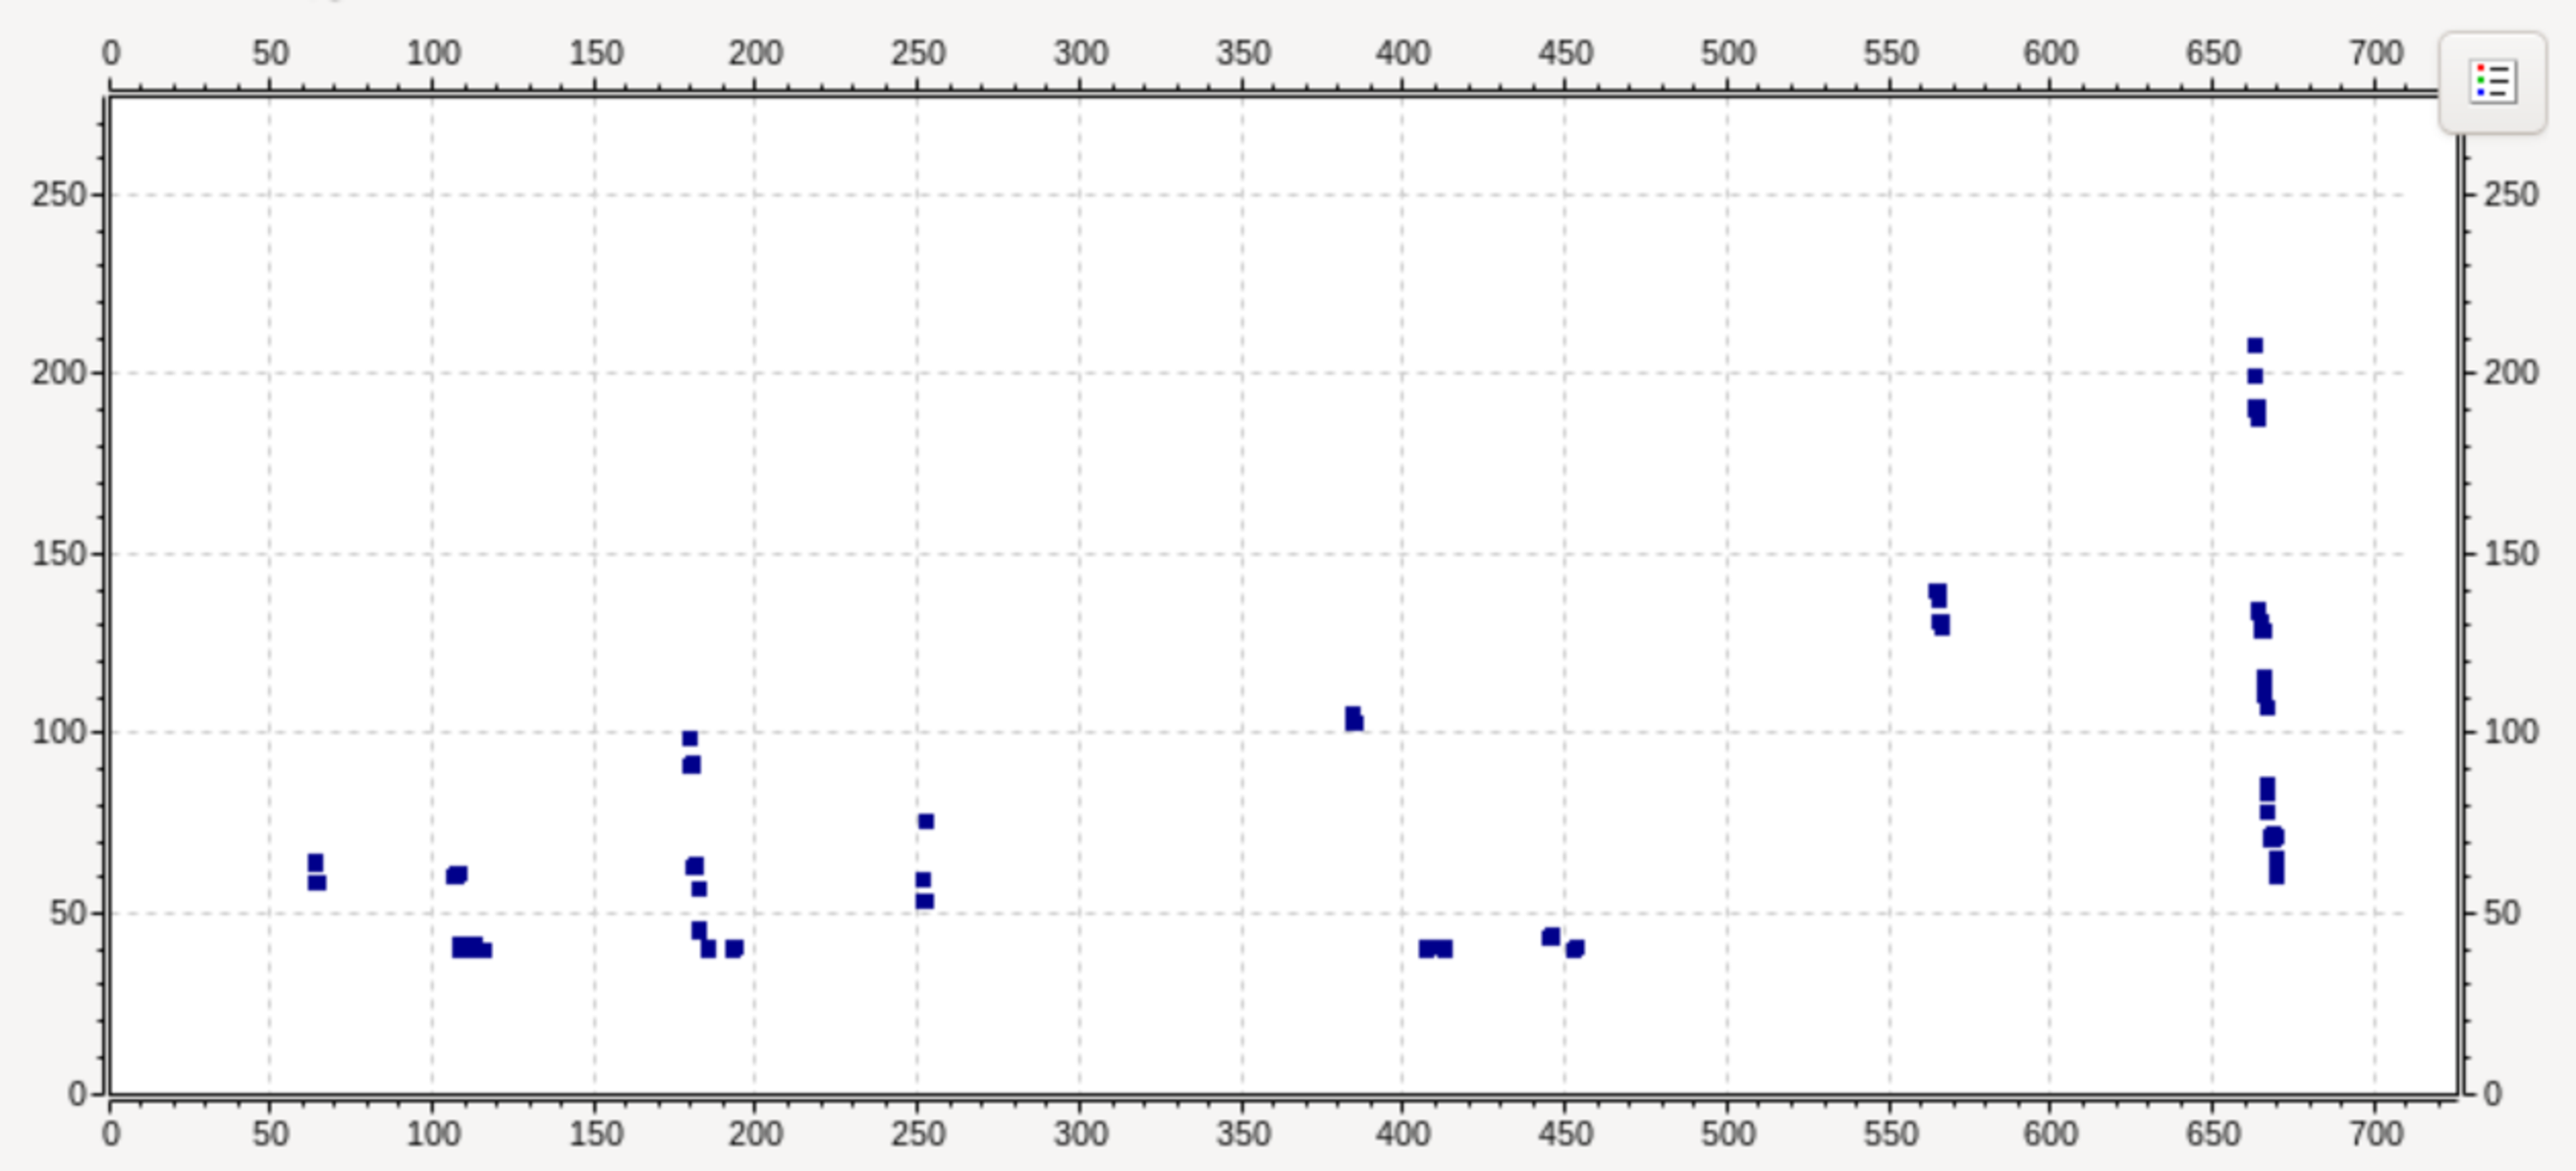
\includegraphics[width=0.7\textheight]{img/thesis_sample_delay_time.pdf}
    \caption{ノード6に向けたBundleの到達遅延の時間変化(地球・火星間のシミュレーション)}
    \label{fig:delay_time_variation_earth_mars}
    \begin{minipage}{\textwidth}
        \raggedright
    \end{minipage}
\end{figure}

\begin{figure}[tbh]
    \centering
    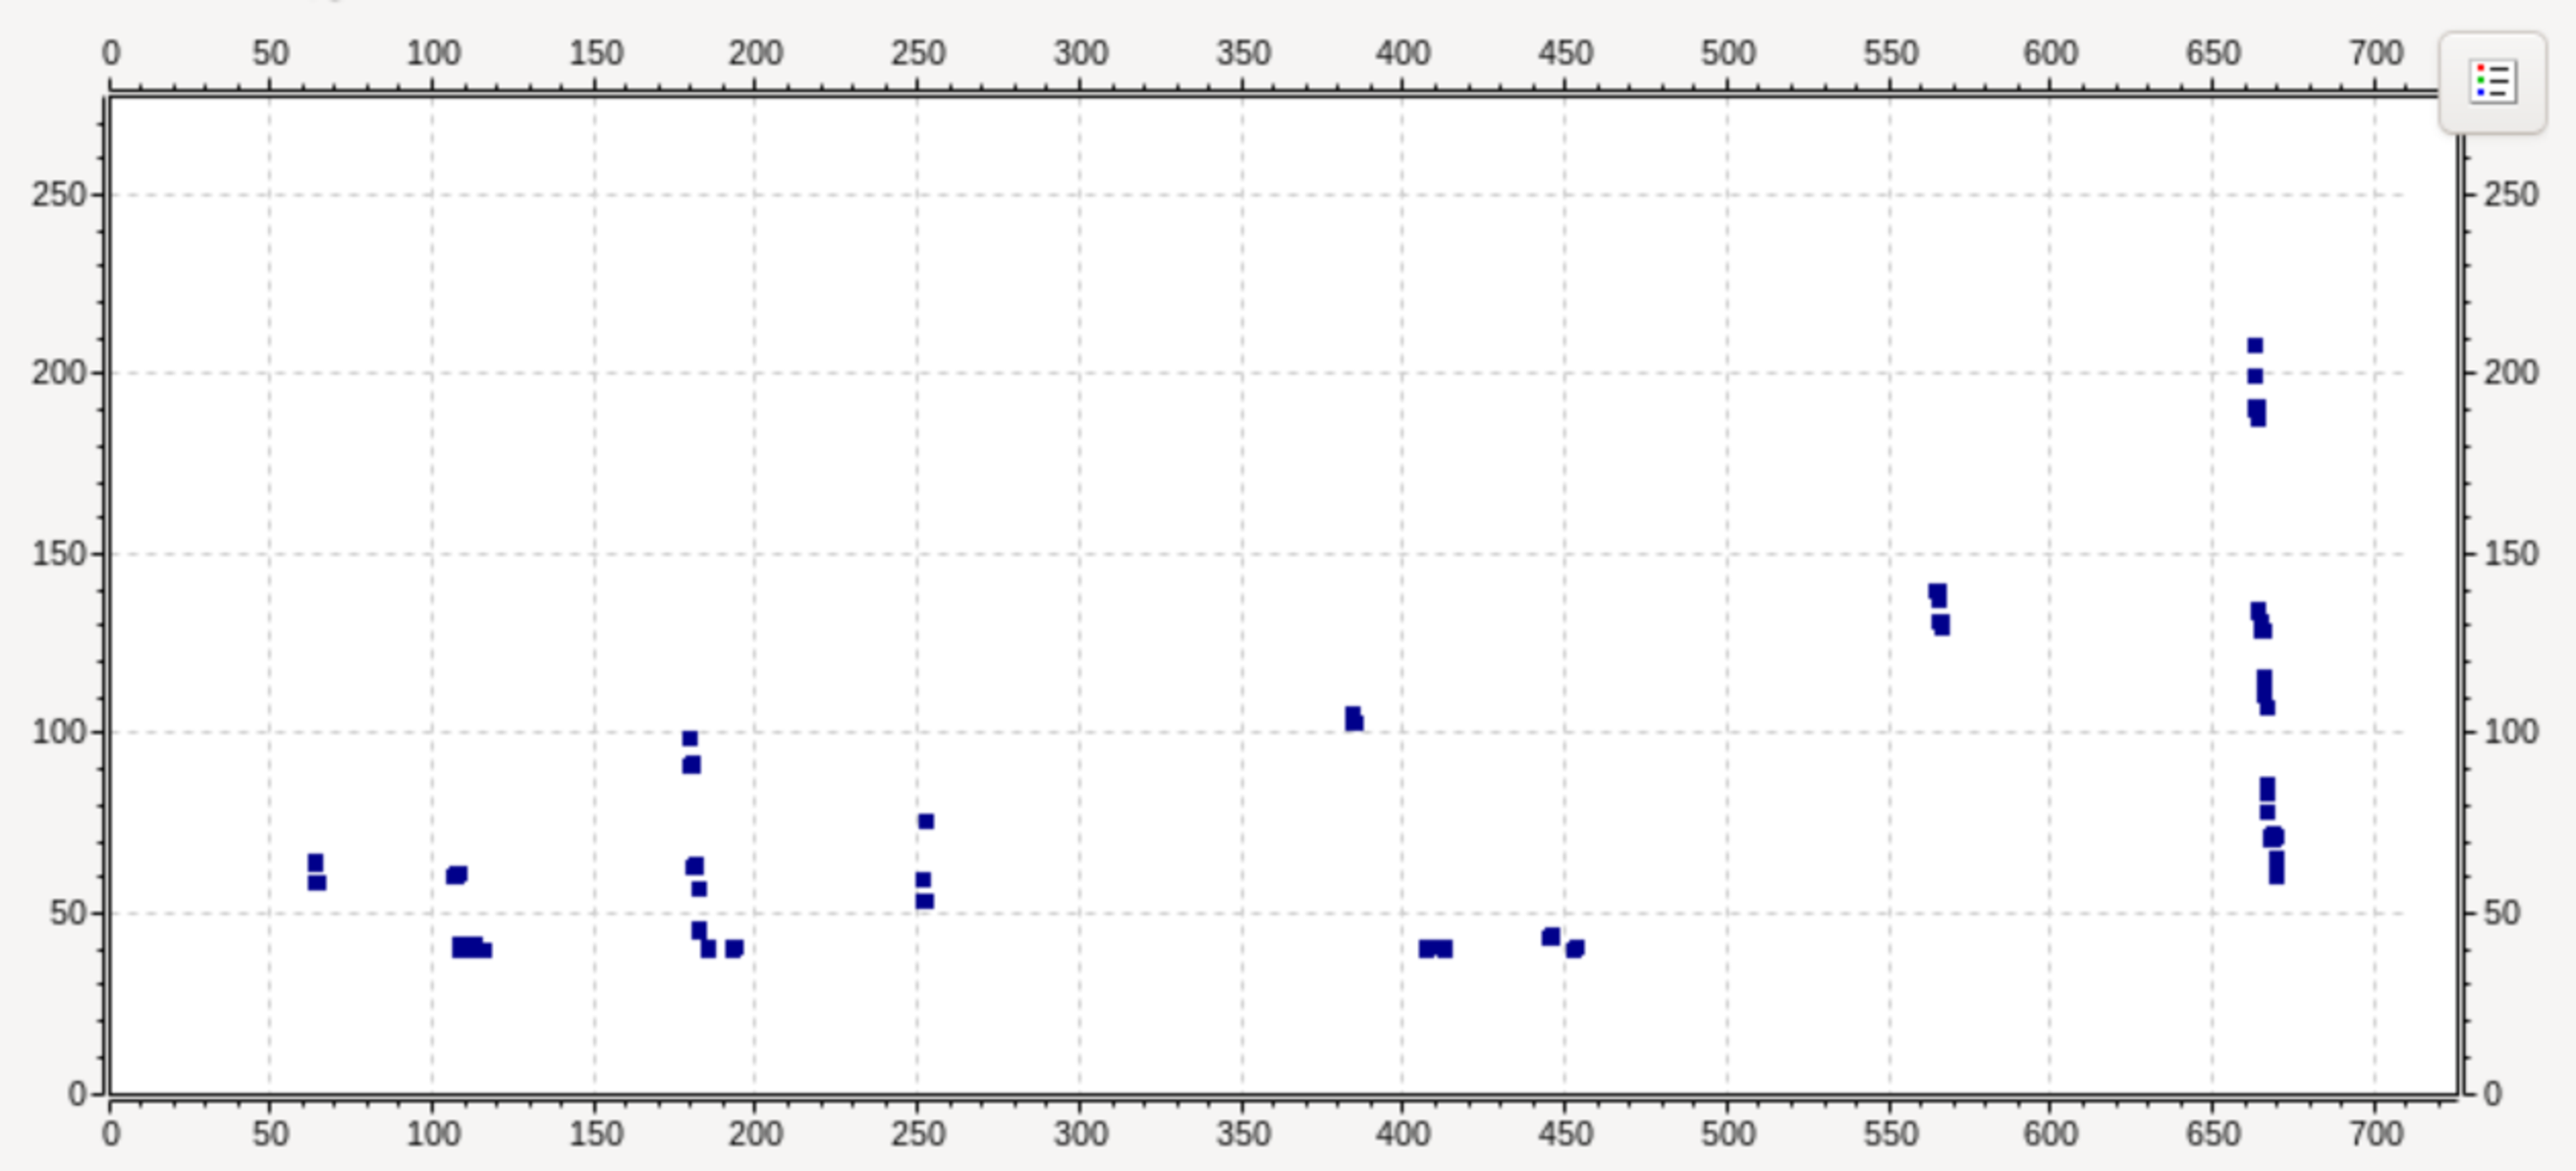
\includegraphics[width=0.7\textheight]{img/thesis_sample_delay_time.pdf}
    \caption{ノード6に向けたBundleの到達遅延の時間変化(火星・火星の衛星間のシミュレーション)}
    \label{fig:delay_time_variation_mars_marssat}
    \begin{minipage}{\textwidth}
        \raggedright
    \end{minipage}
\end{figure}

\subsection{経路収束後の到達遅延}
\label{subsection:経路収束後の到達遅延}
\ref{subsection:要件2}で述べた通り、リンク障害による配送遅延の増加の発生後、
Contact Planの臨時更新を行うと、そのリンク情報がすべてのノードに伝搬し
再計算が行われる時間、すなわち収束までの時間

\begin{figure}[tbh]
    \centering
    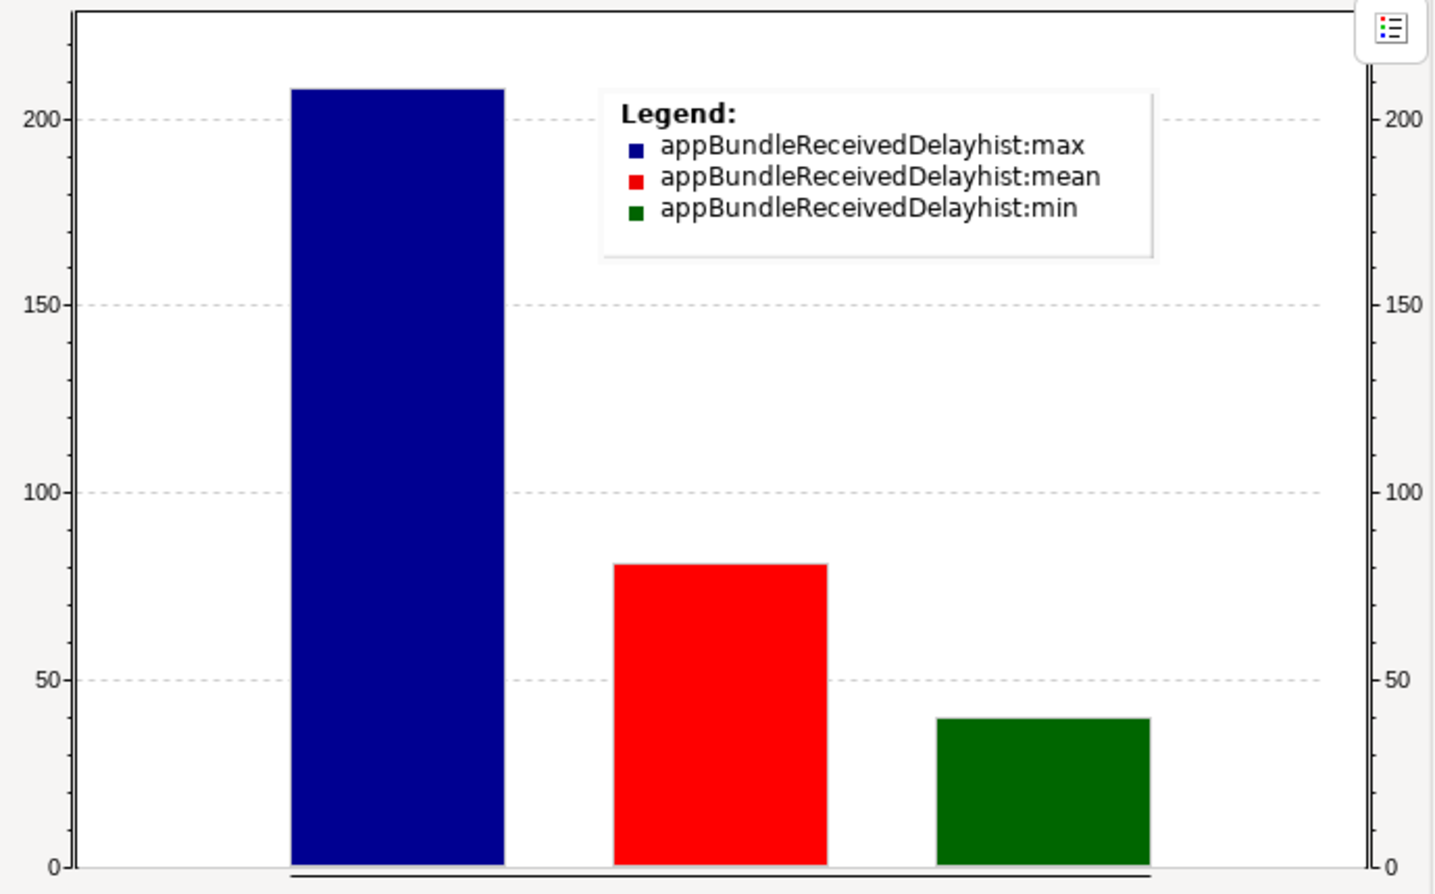
\includegraphics[width=0.7\textheight]{img/thesis_sample_delay_hist.pdf}
    \caption{ノード6に向けたBundleの到達遅延(地球・月間のシミュレーション)}
    \label{fig:total_delay_histgram_earth_moon}
    \begin{minipage}{\textwidth}
        \raggedright
        ノード6における、シミュレーション内での全到達Bundleの到達遅延の時間変化
        \ref{fig:delay_time_variation}同様ノード6のみの到達遅延を示す。
    \end{minipage}
\end{figure}

\begin{figure}[tbh]
    \centering
    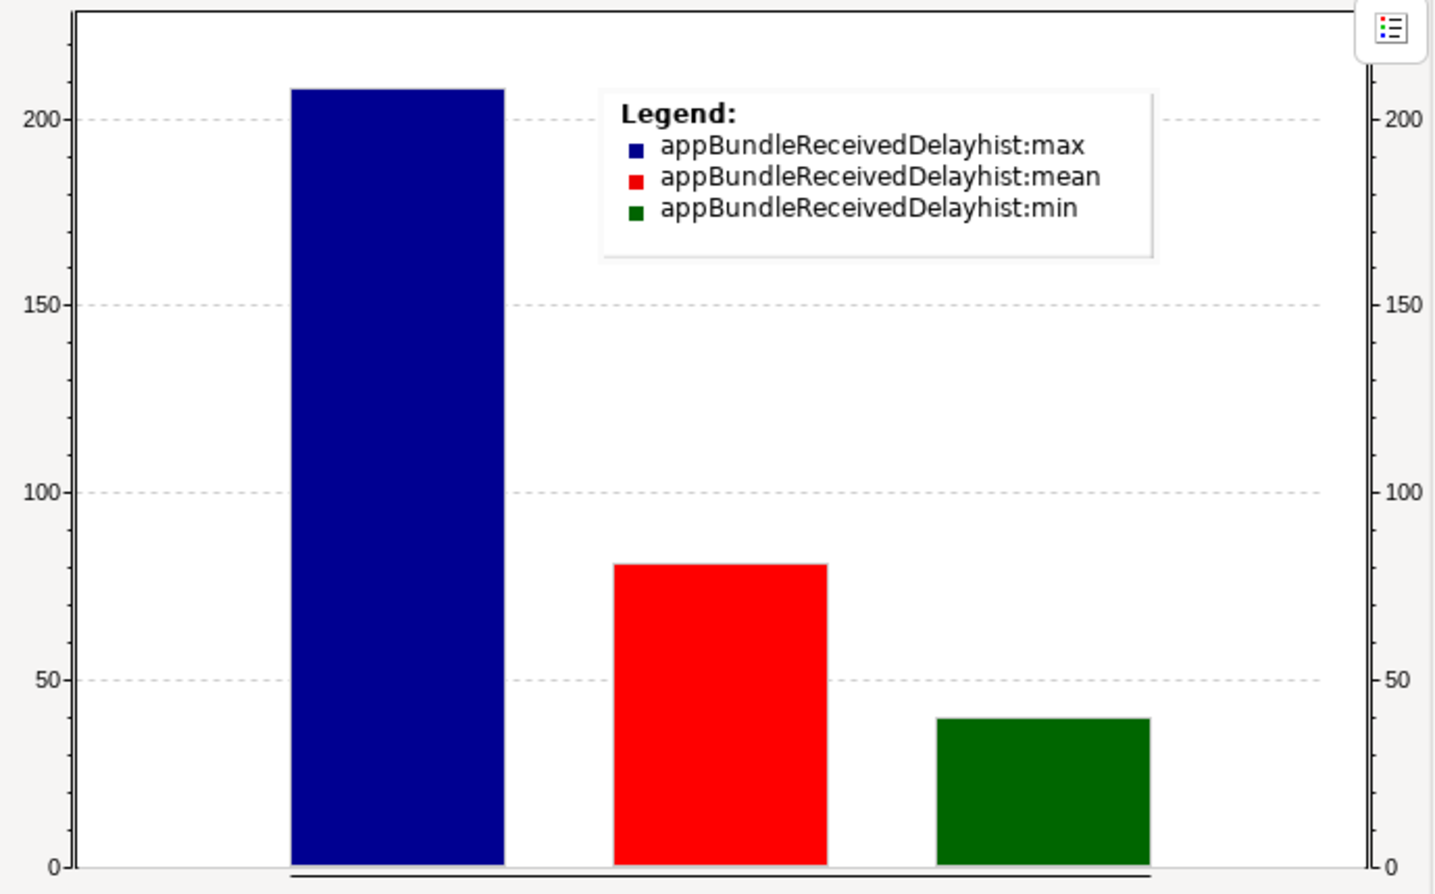
\includegraphics[width=0.7\textheight]{img/thesis_sample_delay_hist.pdf}
    \caption{ノード6に向けたBundleの到達遅延(地球・火星間のシミュレーション)}
    \label{fig:total_delay_histgram_earth_mars}
    \begin{minipage}{\textwidth}
        \raggedright
    \end{minipage}
\end{figure}

\begin{figure}[tbh]
    \centering
    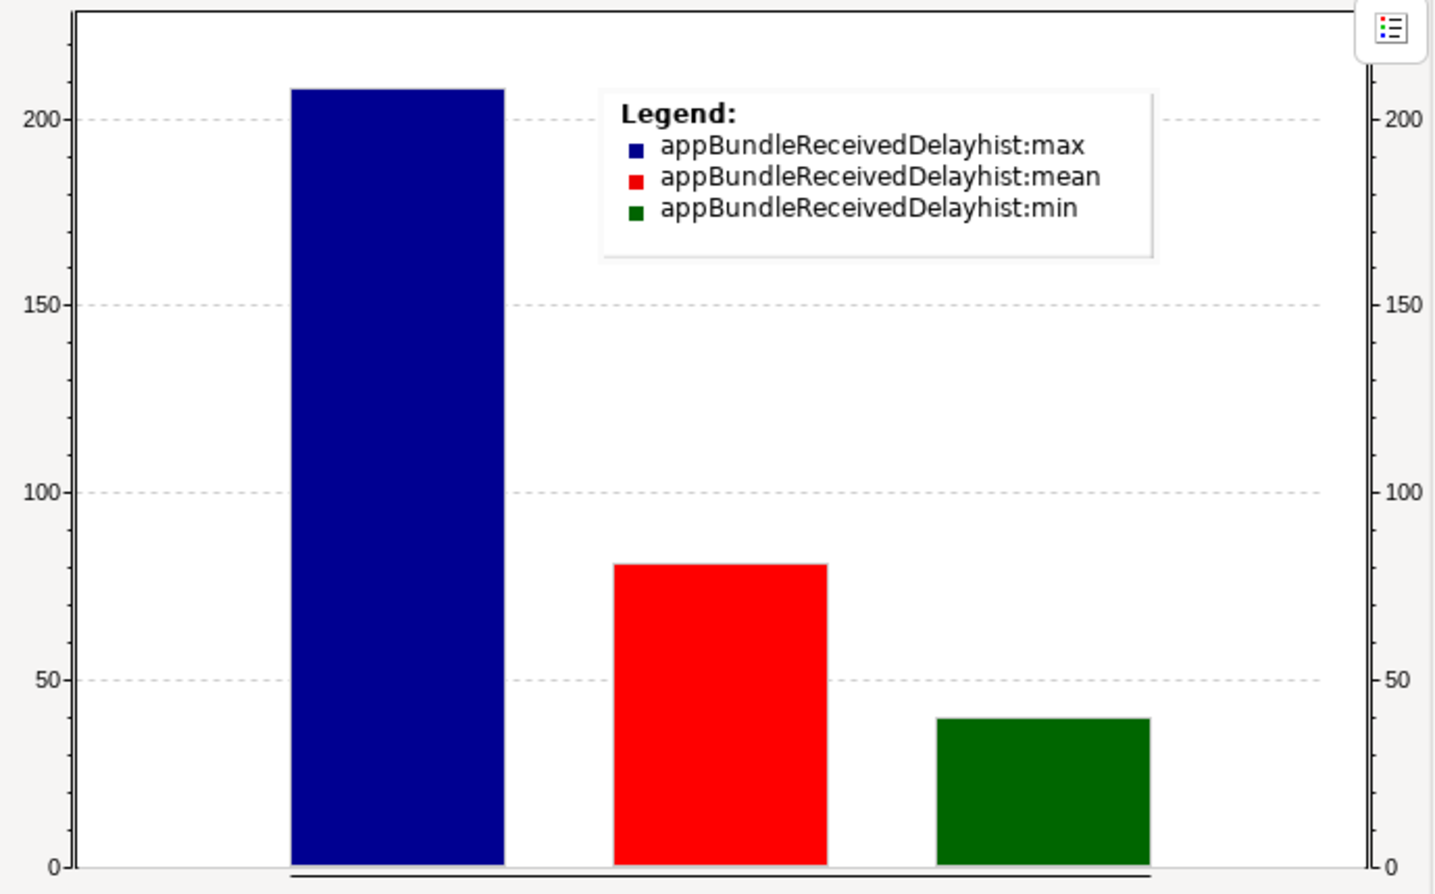
\includegraphics[width=0.7\textheight]{img/thesis_sample_delay_hist.pdf}
    \caption{ノード6に向けたBundleの到達遅延(火星・火星の衛星間のシミュレーション)}
    \label{fig:total_delay_histgram_mars_marssat}
    \begin{minipage}{\textwidth}
        \raggedright
    \end{minipage}
\end{figure}